\begin{figure}
\centering
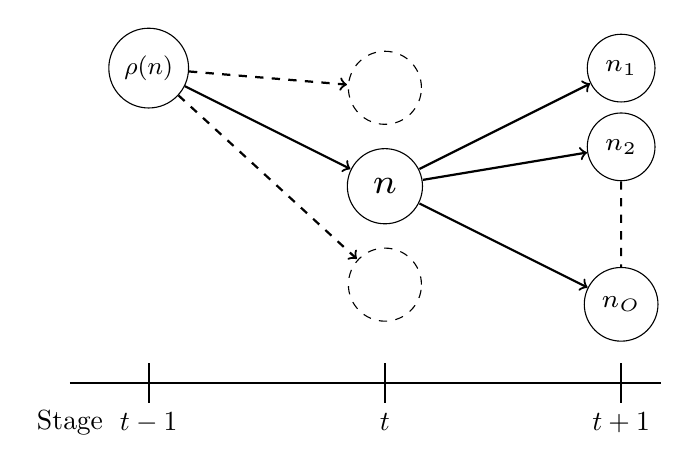
\begin{tikzpicture}

\draw (-1,2.5) node(RHO)[circle,draw]{\small $\rho(n)$ };
\draw (2,2.25) node(NUP)[circle,dashed,scale=2.8,draw]{ };
\draw (2,1) node(N)[circle,scale=1.8,draw]{\scriptsize $n$ };
\draw (2,-.25) node(NDOWN)[circle,dashed,scale=2.8,draw]{ };
\draw (5,2.5) node(N1)[circle,scale=1.3,draw]{\scriptsize $n_1$ };
\draw (5,1.5) node(N2)[circle,scale=1.3,draw]{\scriptsize $n_2$ };
\draw (5,-.5) node(NO)[circle,scale=1.3,draw]{\scriptsize $n_O$ };

\draw[thick,dashed, ->] (RHO) -- (NUP);
\draw[thick,->] (RHO) -- (N);
\draw[thick,dashed, ->] (RHO) -- (NDOWN);
\draw[thick,->] (N) -- (N1);
\draw[thick,->] (N) -- (N2);
\draw[thick,->] (N) -- (NO);
\draw[thick,dashed] (N2) -- (NO);

\draw[thick] (-2,-1.5) -- (5.5,-1.5);
\draw[thick] (-1, -1.75) -- (-1, -1.25);
\draw[thick] (2, -1.75) -- (2, -1.25);
\draw[thick] (5, -1.75) -- (5, -1.25);

\draw(-2,-2) node {Stage};
\draw(-1,-2) node {$t-1$};
\draw(2,-2) node {$t$};
\draw(5,-2) node {$t+1$};

\end{tikzpicture} 
\caption{Stochastic tree for Mixed-Integer Formulation}
  \label{fig:mip}
\end{figure}
